% ======================================================================
\begin{ex}
		\immini{Một tên trộm đang trèo tường để đào thoát bằng một sợi dây như hình minh họa. Trọng lượng của tên trộm này là $\SI{600}{\newton}$. 
			\begin{enumerate}[label=\alph*)]
				\item Xác định lực căng trên mỗi dây.
				\item Nếu điểm treo của sợi dây nằm ngang được đặt ở vị trí cao hơn trên tường thì lực căng của sợi dây bên kia sẽ thay đổi như thế nào?
			\end{enumerate}
		}
		{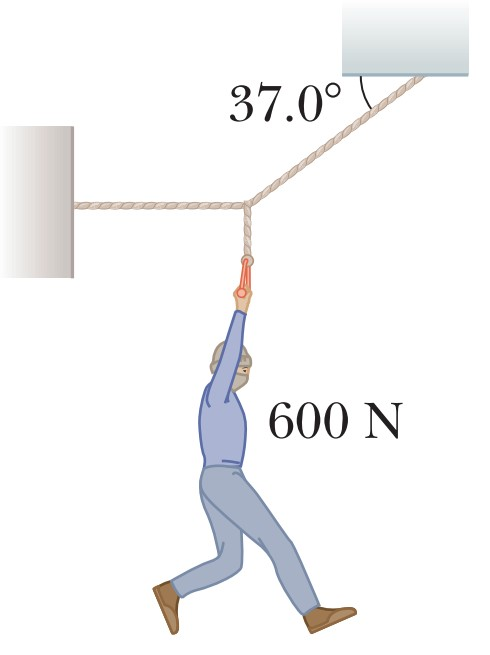
\includegraphics[scale=0.4]{figs/BTMASAT-6}}	
	\loigiai{
	\begin{enumerate}[label=\alph*)]
		\item $T_1=\dfrac{P}{\tan\SI{37}{\degree}}\approx\SI{796}{\newton}$;\\
		$T_2=\dfrac{P}{\sin\SI{37}{\degree}}\approx\SI{997}{\newton}$.
		\item Khi dây nằm ngang, chỉ có thành phần $\vec{T}_{2y}$ trên phương thẳng đứng cân bằng với trọng lực của dây. Khi điểm treo dây được đặt ở vị trí cao hơn trên tường, $\vec{T}_{1}$ đóng góp thêm thành phần $\vec{T}_{1y}$ trên phương thẳng đứng. Do đó, lực căng trên dây $T_2$ giảm đi.
	\end{enumerate}
	}
\end{ex}
% ======================================================================
\begin{ex}
Một bạn học sinh có khối lượng $m=\SI{55}{\kilogram}$ đang thực hiện động tác bật nhảy tại chỗ (jump squat) bằng hai chân trên sàn cứng như hình minh họa bên dưới.
\immini{
	Tại thời điểm $t_0=0$, học sinh đạt độ cao cực đại và vận tốc bằng 0. Tại thời điểm $t_1$, học sinh này rơi xuống chạm vào mặt sàn bằng hai chân, trọng tâm thân người di chuyển đoạn $h=\SI{0.65}{\meter}$ so với trọng tâm tại thời điểm $t_0$. Để giảm lực tác động lên khớp gối và cột sống trong quá trình tiếp xúc với sàn, bạn này thực hiện động tác gập gối sao cho giữa các thời điểm $t_1$ và $t_2$ trọng tâm của bạn ấy hạ xuống một khoảng $\Delta h=\SI{0.36}{\meter}$.  Coi quá trình bạn học sinh rơi trong không khí là rơi tự do. Lấy gia tốc rơi tự do $g=\SI{10}{\meter/\second^2}$.
}
{\vspace{-0.5cm}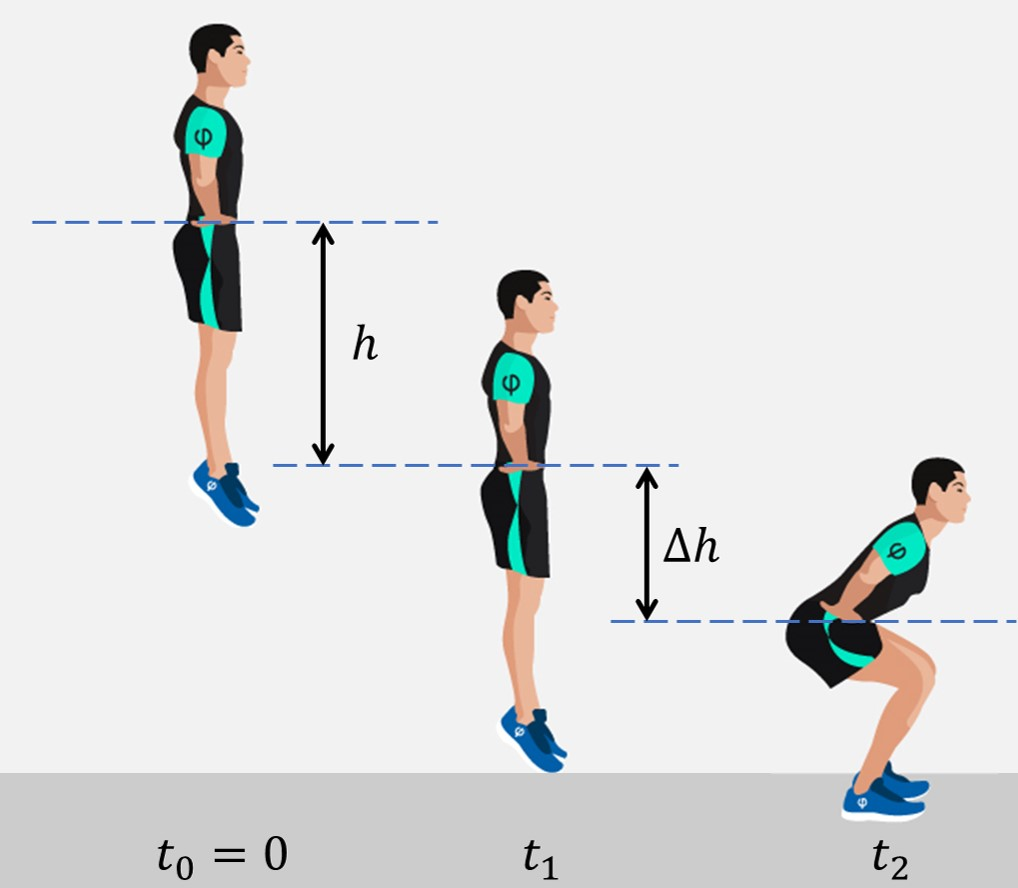
\includegraphics[scale=0.3]{figs/D10-HKI-KTTX2-001-5}}	
	\begin{enumerate}[label=\alph*)]
	\item Dựa vào kiến thức đã học, em hãy trình bày cơ sở khoa học của việc gập gối của bạn học sinh trong trường hợp ở trên.
	\item Xác định tốc độ của bạn học sinh khi ngay trước khi chạm đất.
	\item Xác định độ lớn lực cản trung bình của sàn nhà tác dụng lên chân bạn học sinh.
\end{enumerate}
	\loigiai{
\begin{enumerate}[label=\alph*)]
	\item Khi chân người vừa chạm đất, thân trên vẫn tiếp tục di chuyển xuống dưới theo quán tính và tạo áp lực lên khớp gối. Do đó, việc gập gối góp phần làm tăng thời gian 
\end{enumerate}
	}
\end{ex}